% Created 2020-03-05 Thu 17:01
% Intended LaTeX compiler: pdflatex
\documentclass[presentation]{beamer}
\usepackage[utf8]{inputenc}
\usepackage[T1]{fontenc}
\usepackage{graphicx}
\usepackage{grffile}
\usepackage{longtable}
\usepackage{wrapfig}
\usepackage{rotating}
\usepackage[normalem]{ulem}
\usepackage{amsmath}
\usepackage{textcomp}
\usepackage{amssymb}
\usepackage{capt-of}
\usepackage{hyperref}
\usetheme{UoB}
\author{Mark Blyth}
\date{\textit{[2020-03-09 Mon]}}
\title{A continuum approach to neuron modelling}
\hypersetup{
 pdfauthor={Mark Blyth},
 pdftitle={A continuum approach to neuron modelling},
 pdfkeywords={},
 pdfsubject={},
 pdfcreator={Emacs 26.3 (Org mode 9.1.9)}, 
 pdflang={English}}
\begin{document}

\maketitle

\section{Background}
\label{sec:org7f31c62}
\begin{frame}[label={sec:orga6d73b5}]{Overview}
\begin{itemize}
\item Challenges with using the MEA
\item Possible solutions (network- and microfluidic-based methods)
\item A better solution (continuum)
\item Literature precedent
\end{itemize}
\end{frame}

\section{Challenges}
\label{sec:org433c7db}
\begin{frame}[label={sec:org2a7da5b}]{Main challenge with the MEA}
\begin{itemize}
\item Loss of spatial resolution, since we can no longer measure and perturb individual cells
\item Emergent behaviours mean we can't study dynamics of individual neurons; would have to study network dynamics instead
\item Too many unknowns to build a realistic network model\ldots{}
\end{itemize}
\end{frame}

\begin{frame}[label={sec:org898d8af}]{Issues with the network model}
\begin{itemize}
\item No geometric information 
\begin{itemize}
\item We can make a model of neuron networks, but there's no easy way to relate an agent in the network to the position of a living cell
\item This matters, as we can't predict the spatial dynamics, and therefore the effects of stimulating each electrode, without this information
\end{itemize}
\item No topological information
\begin{itemize}
\item We don't know who connects to who, in our neuron network
\item This means we can't produce an accurate network model
\end{itemize}
\item Too many equations for simulations
\begin{itemize}
\item 200,000 neurons is too many to simulate!
\end{itemize}
\item Too many parameters to accurately determine
\begin{itemize}
\item Even just coupling strength adds between 200,000 and 40,000,000,000 (200,000\(^{\text{2}}\)) extra parameters to the model
\end{itemize}
\end{itemize}
\end{frame}

\begin{frame}[label={sec:org27bd80a}]{Some possible solutions}
\begin{itemize}
\item Constrain the network geometry using on-chip microchannels
\begin{itemize}
\item This has been done in the literature
\item Doesn't tell us much about connection strengths
\item Would be a very hard device to make
\item Requires making another new device
\end{itemize}
\item Use synchronisation-based network models
\begin{itemize}
\item Changing one of 200,000 network connection strengths probably won't change much in the dynamics
\item Can use this lack of sensitivity to make simpler models of neuron synchronisation
\item But, this synchronisation models won't work for any case other than synchronisation (limits the dynamics with specific assumptions)
\end{itemize}
\end{itemize}
\end{frame}

\begin{frame}[label={sec:org1041f69}]{A proposed alternative}
\begin{itemize}
\item Assume we have an arbitrarily large number of neurons
\item Every neuron connects to every other neuron within its local neighbourhood
\item Treat it as a continuum (neural field, rather than point neurons)
\item Build a PDE model
\end{itemize}
\end{frame}

\begin{frame}[label={sec:org494a480}]{Benefits of a continuum model (1)}
\begin{itemize}
\item No need to know the network geometry; any given `neuron' is identified by its point in the domain
\item No need to define a network topology; every `neuron' interacts locally with those in its neighbourhood
\item Far fewer parameters are required to characterise the system
\begin{itemize}
\item Don't need to specify a set of parameters for each agent in a network system
\end{itemize}
\item Becomes tractable to study much more sophisticated dynamics than with the network model (beyond simple synchronisation!)
\item We no longer care about what individual cells are doing, and can therefore get away with the lower spatial resolution of the electrodes
\begin{itemize}
\item Instead, we're measuring the average continuum value across some small region, which is a sufficient measurement; don't need to know the state of every neuron in the network
\end{itemize}
\end{itemize}
\end{frame}

\begin{frame}[label={sec:org849ae19}]{Benefits of a continuum model (2)}
\begin{itemize}
\item No need to individually perturb single neurons - it suffices to model a current input across some subdomain of the PDE's space
\item Microfluidic electrodes have a very natural mathematical interpretation
\begin{itemize}
\item For an accurate model, neurons can be thought of as `solving' the continuum PDE across their network
\item Numerical methods for solving the model would typically use orthogonal collocation
\item A set of meshpoints are defined, and orthogonal basis functions are chosen such that they solve the PDE at those mesh points
\item The electrodes are therefore a physical analog of these collocation mesh points!
\item Very natural transition between numerical methods, and physical experiments
\end{itemize}
\end{itemize}
\end{frame}

\section{Literature precedent}
\label{sec:org60905c8}
\begin{frame}[label={sec:orgcdcd768}]{Literature precedent}
\begin{itemize}
\item There's models for neural fields
\begin{itemize}
\item Bressloff, Paul C. "Spatiotemporal dynamics of continuum neural fields." Journal of Physics A: Mathematical and Theoretical 45.3 (2011): 033001.
\item Seems to be based on some rather dubious assumptions (rate-based networks, assume SNIC neurons)
\end{itemize}
\item There's also cable models for spatially extended neurons
\begin{itemize}
\item Designed to model signal propagation down an axon
\item Could possibly produce a 2d spatially extended system as a continuum model?
\item I don't yet know how important the synaptic dynamics are on continuum dynamics
\end{itemize}
\end{itemize}
\end{frame}
\begin{frame}[label={sec:orge0ab2e0}]{The Belousov-Zhabotinksy reaction}
Chemical reaction, displaying complex dynamics away from equilibrium.
I claim it behaves in the same way as neurons:
\begin{itemize}
\item Consider reactants as `ions inside a neuron'
\item Consider products as `ions outside a neuron'
\item Consider catalyst concentration as membrane potential
\begin{itemize}
\item Stimulates the transition of reactants into products (and reverse)
\item Equivalently, stimulates the movement of ions into a cell (and out of it)
\end{itemize}
\end{itemize}
Dynamics of the BZ reaction are therefore analogous to those of a neural continuum.

This is analogy interesting, as there's lots of research on the various behaviours of the BZ reaction that could be reapplied to predict dynamics of a large neural population.
But, interestingly\ldots{}
\end{frame}

\begin{frame}[label={sec:org4182f6d}]{Controlling the BZ reaction}
\begin{itemize}
\item The BZ reaction is a continuum system.
\item Methods have been demonstrated for tracking its dynamics, suggesting that similar approaches may work for neurons.
\item These follow an OGY/ ETDF style approach.
\end{itemize}

Petrov, Valery, Michael J. Crowley, and Kenneth Showalter. "Tracking unstable periodic orbits in the Belousov-Zhabotinsky reaction." Physical review letters 72.18 (1994): 2955.

Petrov, Valery, Michael F. Crowley, and Kenneth Showalter. "An adaptive control algorithm for tracking unstable periodic orbits." International Journal of Bifurcation and Chaos 4.05 (1994): 1311-1317.
\end{frame}

\begin{frame}[label={sec:orgb251ebe}]{Epilepsy, coherent structures, and Turing instabilities}
\begin{itemize}
\item Epilepsy is characterised by waves travelling across the surface of the brain [SOURCE?]
\item Travelling waves are a type of `coherent structure' (some structure that appears and persists in the dynamics)
\item More generally, Turing patterns refer to the appearance of coherent structures in reaction-diffusion systems (like BZ reaction!)
\item Since we've added a spatial domain, we now have new ways to bifurcate
\begin{itemize}
\item Lose stability in temporal dimension - traditional bifurcation
\item Lose stability in spatial dimension - Turing instability
\end{itemize}
\item Turing patterns and instabilities form new bifurcations we could control and test for
\begin{itemize}
\item \ldots{}possibly bifurcations that lead to epileptic dynamics?
\end{itemize}
\end{itemize}
\end{frame}

\begin{frame}[label={sec:org31e46a7}]{Studying continuum models}
\begin{itemize}
\item Turing patterns are a very well studied area - lots of literature to draw from
\item There's also lots of literature on PDEs
\item (I conjecture) it would be considerably easier to study bifurcations in the PDEs than in a massive network
\end{itemize}
\end{frame}

\begin{frame}[label={sec:orgd7db8ae}]{Interlude for pretty pictures}
\begin{columns}
\begin{column}{0.5\columnwidth}
\begin{center}
\includegraphics[width=.9\linewidth]{./BZ.jpg}
\end{center}
\end{column}

\begin{column}{0.5\columnwidth}
\begin{center}
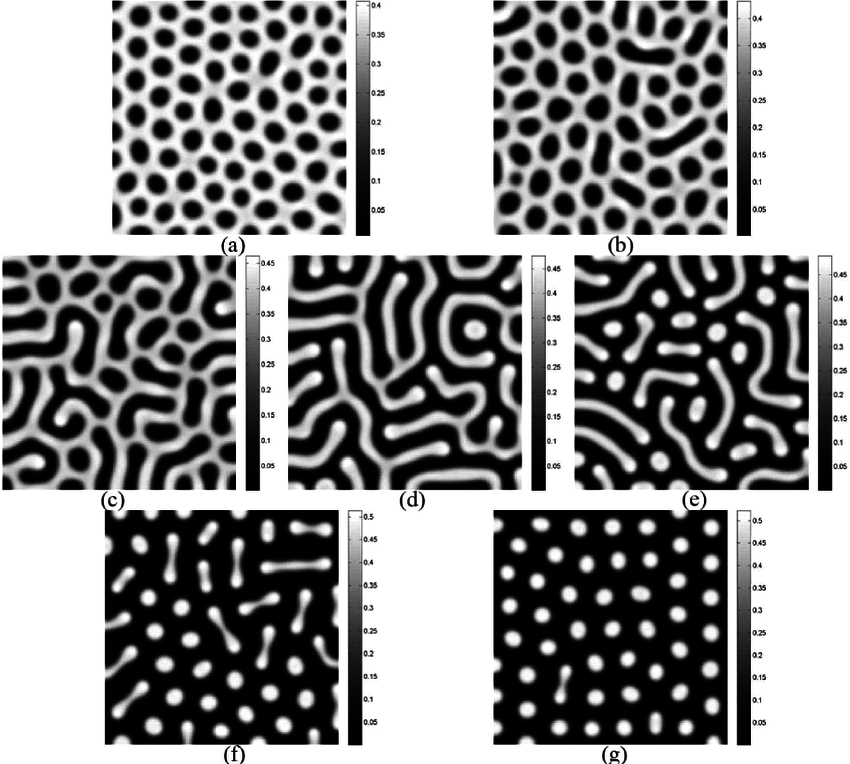
\includegraphics[width=.9\linewidth]{./turingpatterns.png}
\end{center}
\end{column}
\end{columns}
\end{frame}

\begin{frame}[label={sec:org363b05a}]{Handy to know\ldots{}}
Alan is an expert in this area.
\end{frame}

\section{Plan suggestion}
\label{sec:orgd25d35c}
\begin{frame}[label={sec:org6c6269e}]{Some issues}
\begin{itemize}
\item The continuum model discussed in previous review is rate-based; doesn't generalise to arbitrary neurons, only good for cortical (SNIC) neurons
\item A spatially extended cubic Lienard model would give the dynamics of arbitrary neuron populations, if and only if synaptic dynamics are non-critical
\end{itemize}
\end{frame}
\begin{frame}[label={sec:org588e70e}]{Possible project plan}
\begin{itemize}
\item Produce a neuron normal form model
\begin{itemize}
\item Krasi's cubic Lienard + a slow subsystem
\end{itemize}
\item Generate a neural continuum model from a spatially extended normal form
\item Analyse bifurcations etc. in the model, to get an idea of what the actual cells will do
\item Develop a CBC approach to track those bifurcations
\end{itemize}

Note that a spatially extended neuron model might not be sufficient; the review cited earlier would be a good place to start on understanding good continuum models.
\end{frame}

\begin{frame}[label={sec:org6f0b20c}]{Possible project plan}
Nice but not necessarily essential:
\begin{itemize}
\item Bigger MEA (more cells = more like a continuum)
\item More electrodes (more collocation meshpoints = more accurate model)
\end{itemize}
\end{frame}
\end{document}
